\chapter{Simulation-free training of continuous normalising flows}
\label{ch:simulation-free}
\section{From simulation-based to simulation-free training}
\Acfp{CNF} connect a source distribution to a data distribution through a depth-dependent vector field. Training through numerical integration can require repeated forward and backward solves. Simulation-free objectives instead sample intermediate states from a prescribed probability path and regress an available conditional target. Sampling and likelihood evaluation can still require numerical integration.

This chapter organises these methods around probability paths, prediction targets, conditioning, and inference. Throughout, $u=0$ denotes the data endpoint and $u=1$ the source endpoint; generation proceeds towards decreasing $u$.

Figure~\ref{fig:path-overview} provides a visual overview of the paths considered below: \acf{MR-VP}, \acf{SB-VE}, \acf{SB-SV}, and the linear interpolation paths used for flow matching (labelled \acs{ICFM}, for \acl{ICFM}, in the figure).
\begin{figure}[p]
\centering
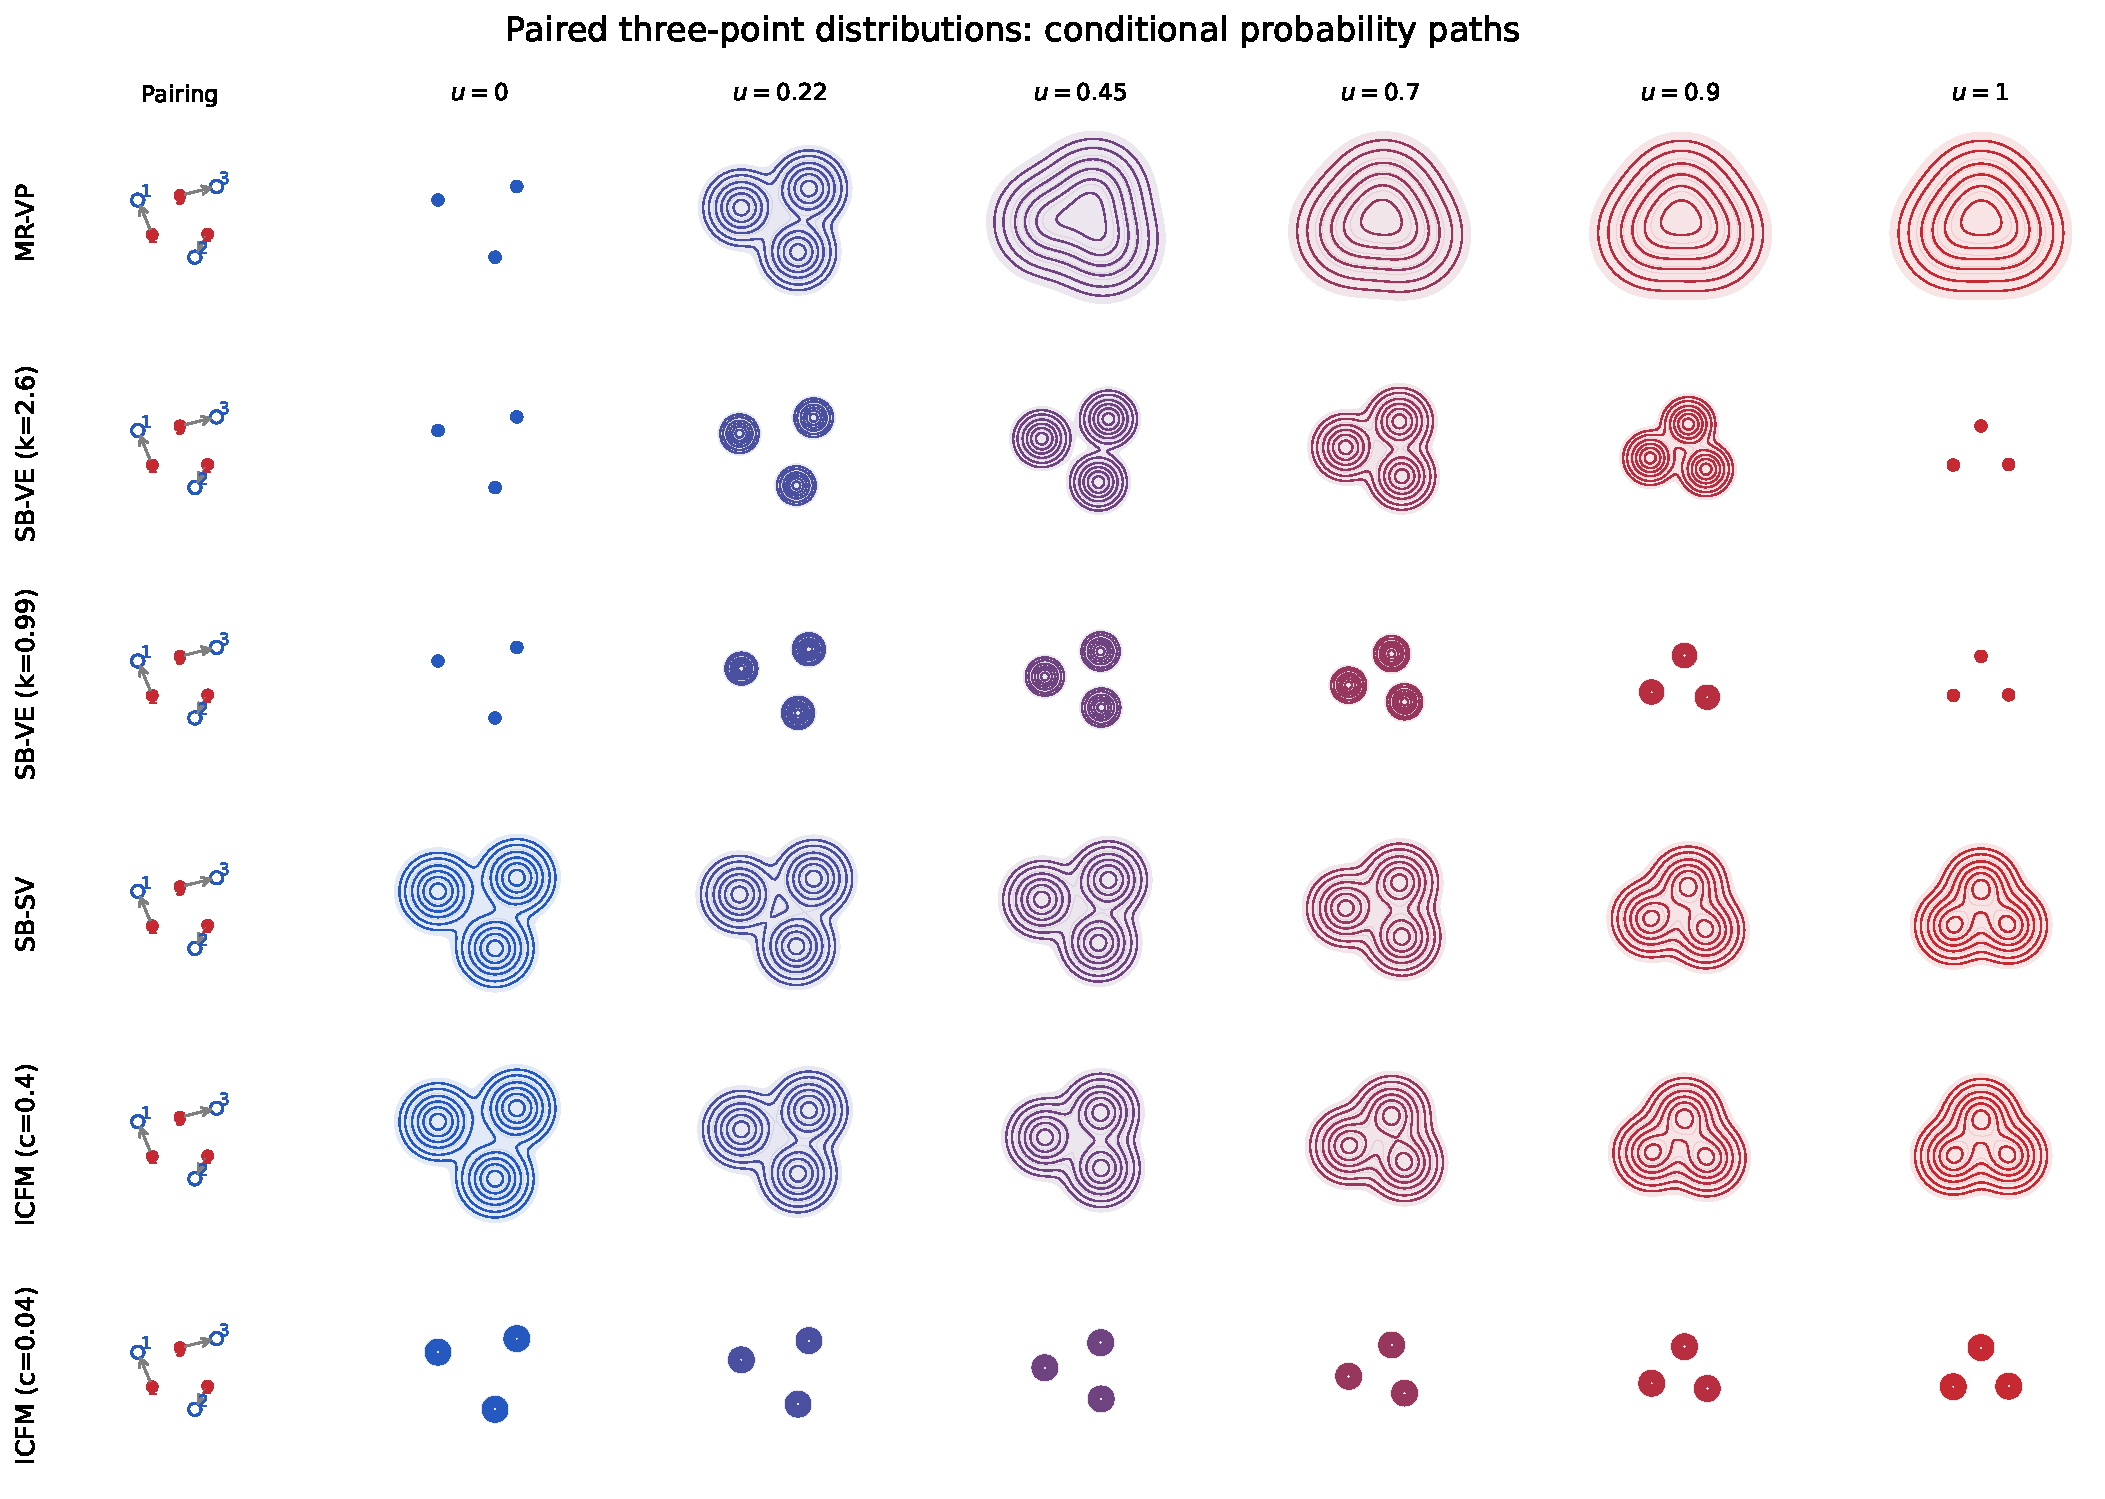
\includegraphics[width=\linewidth]{plots/simulation_free/ripple_paths_paired_diracs.pdf}
\caption{Probability-path overview for three paired target and source points. Each row shows density contours at increasing depth $u$; generation proceeds from right to left. \acs{MR-VP} approaches a Gaussian mixture about the source points, \acs{SB-VE} has exact point-mass endpoints, and \acs{SB-SV} and the flow-matching paths retain Gaussian smoothing at both endpoints. The two \acs{SB-VE} schedules and two flow-matching variances illustrate their effects on the intermediate densities. Here \acs{ICFM} denotes the linear, constant-variance path form used with the displayed pairing, rather than independent endpoint sampling.}
\label{fig:path-overview}
\end{figure}
\clearpage
\section{Probability paths and endpoint distributions}
\label{sec:probability-paths}

The central tool for simulation-free training is the definition of a probability path $p_u$. A path is a depth-varying density, which may be marginal or conditional. The conditional paths considered here are Gaussian, with intermediate states $\rmX_u\sim p_u$ sampled as
\[
\rmX_u=\rmM_u+\tSigma(u)^{1/2}\rmZ,\qquad \rmZ\sim\gN(\bm0,\tI).
\label{eq:xu_sample}
\]
The mean $\rmM$ and covariance $\tSigma$ depend on the chosen construction and its conditioning variables. A typical mean function is an interpolation of endpoint samples such as
\[
\rmM(u,\rmX,\rmY)\coloneqq a(u)\rmX + b(u)\rmY,
\]
where $a(0)=b(1)=1$ and $a(1)=b(0)=0$. When $\rmY=0$, the marginal at $u=1$ becomes similar to a standard normal $p_1(\rmX_1)\simeq\gN(\bm0,\tSigma)$. The boundaries $p_0$ and $p_1$ are known as the \textit{target} and \textit{source} distribution respectively. A path derived from a data endpoint is known as a \textit{conditional} path $p_u(\rmX_u|\rmX_0)$, which may also be conditioned on $\rmX_1$ as well.

For paired endpoints, their joint law is denoted by $\pi(\rmX,\rmY)$. This contrasts the original idea of a normalising flow, as now the flow is a coupling between two potentially non-normal distributions. Despite this, such flows still lie within the \acs{CNF} framework.

Conditional paths are used as a reference for learning a marginal path. This aspect is what makes training simulation-free, as the conditional path can be sampled at any $u$ during training, and the marginal path is optimised for any $u$. This format is useful, and is discussed in \secref{sec:learning-objectives}.

A contrast simulation-free training brings is through the optimisation objective. When simulating the \acs{CNF}, likelihood is maximised directly, and the learnt path is a result of the optimisation algorithm. A probability path instead acts as a target in which a sufficiently trained estimator can retrieve the data marginal. Yet, this is achieved by learning the probability path rather than likelihood maximisation. A useful feature of simulation-free training is that the likelihood density is still tractable through the \acf{ICOV} formula.

These paths typically take the form of a closed expression of a differential equation, as this guarantees that there is a valid trainable vector field. Another common factor is the use of Gaussian probability paths. Although this may seem as an incorrect assumption of the underlying data, by considering the data as a mixture of Gaussians centred at the data points, the smaller the variance of each Gaussian, the closer to the data distribution the path endpoint becomes.

Score-based diffusion models were first developed as a method for training a standard \acs{CNF}, but many proposed modifications have been made to support extended tasks and data such as conditional generation and paired endpoints. On the other hand, Schr\"odinger bridges specify a path problem with endpoint constraints and reference dynamics e.g. go from point A to point B and follow a diffusion-like path. Finally, flow matching also specify a path between endpoints, but no restrictions on the dynamics, thus allowing straight-line paths, which are optimal in the sense that they require the least amount of movement.


The next sections detail the mechanics of these probability paths and how to construct them. The order these are presented in follows the chronology of ``breakthrough'' findings. First diffusion models proved that \acfp{SDE} can be used simulation-free training of \acsp{CNF} with a tractable log-likelihood, then \acfp{SB} use forward-backward \acsp{SDE} for exact-endpoint interpolation, finally flow-matching shows a generalised view through \acfp{ODE}. A key observation made in this thesis is the amount of stochasticity each method has, and its impact on training and sampling.

Simulation-free training avoids numerical integration when constructing the regression objective. Likelihood evaluation generally still requires integrating the learned dynamics and their divergence, as described in \secref{sec:likelihood-evaluation} and examined empirically in \chapref{ch:ll}.

\subsection{Diffusion paths}
\label{sec:diffusion-paths}

Recall that the goal of a \acs{CNF} is to learn a probability path between a source distribution and target distribution. This is formalised as a time varying probability path with boundaries at the desired distributions e.g. $\gN(\bm0,\tSigma)\rightarrow\pdata$. As indicated earlier, the reverse of this path can be described as a diffusion process. Starting from a structured initialisation at $u=0$, the Wiener process $\rmW$ shifts points over time, and at the terminal time $u=1$ the distribution has a similar density to a normal distribution.
The formal description of this begins with an It\^o \acs{SDE}
\[
\dd\rmX \coloneqq \rmF(\rmX)\dd u + g(u)\dd\rmW_u,
\]
where an initial value at $u=0$ is sampled from the data $\rmX_0\sim\pdata(\rmX_0)$ and at $u=1$ the probability path $p_u$ becomes similar to a normal. Any intermediate and final samples can be computed with the following solution
\[
\rmX_u = \rmX_0 + \int_0^u\rmF(\rmX_s,s)\dd s + \int_0^ug(s)\dd \rmW_s,
\label{eq:sdesolv}
\]
either with black-box \acs{SDE} solvers or in closed form.

The reverse process plays a central role to finalising the \acs{CNF} construction, which is written by the result of \cite{andersonReversetimeDiffusionEquation1982}
\[
\dd\rmX = \left[\rmF(\rmX) - g(u)^2\nabla\log p_u(\rmX)\right]\dd u + g(u)\dd\bar\rmW_u,
\label{eq:sderev}
\]
where $\bar\rmW_u$ is the reverse Wiener process. The gradient of the log-density $\nabla\log p_u(\rmX_u)$ is known as the score, and models that estimate it are known as score-based generative models.

Of course, the marginal score at any point $u$ is unknown. However, a path may have a conditional score $\nabla\log p_u(\rmX_u|\rmX_0)$ if the endpoint sample $\rmX_0$ is known e.g. by sampling the data. A standard method is use a conditional path $p_u1(\rmX_u|\rmX_0)$ and score and then learning a neural estimator to replace the conditional. This all begins with a defined conditional path, which is presented next.



\subsection{Mean reversion and variance preservation}
\note{Image and speech example to show what adding noise looks like?}
\ainote{Yes: a small figure with one image and one Mel-spectrogram at the same four depths would connect the Gaussian examples to the thesis applications. Generate each panel from the stated forward marginal, using a fixed noise draw within each row so that changes reflect depth. State the data normalisation, noise schedule, and reversion mean; use fixed display scales across depths. For speech, label this as noise in acoustic-feature space, since it is not equivalent to adding background noise to a waveform.}
\begin{figure}[tbp]
\centering
\subfigure[Common conditioning mean $Y=0$: standard-normal source]{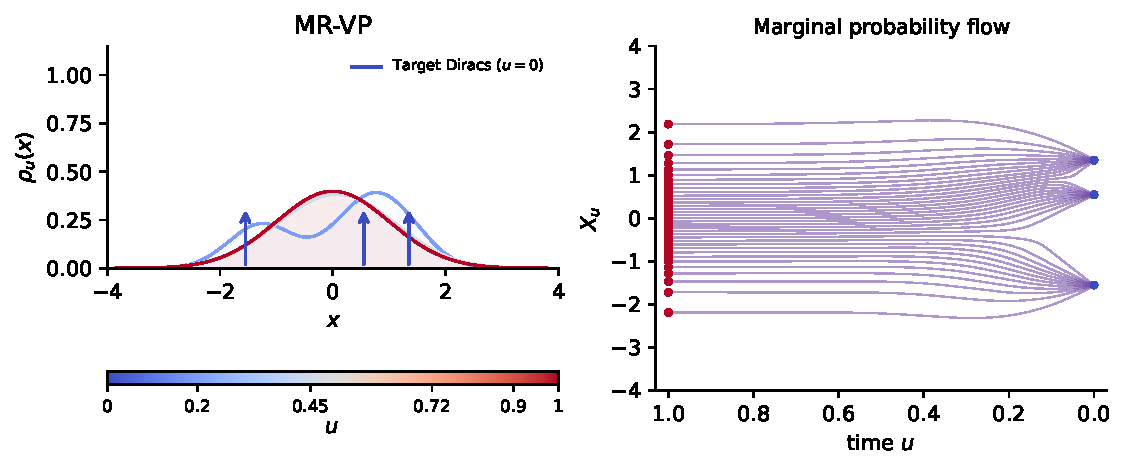
\includegraphics[width=0.95\linewidth]{plots/simulation_free/bridge_1d_mr_vp_normal.pdf}\label{fig:mrvp-normal}}
\par\medskip
\subfigure[Paired conditioning points $y_i$: Gaussian-mixture source]{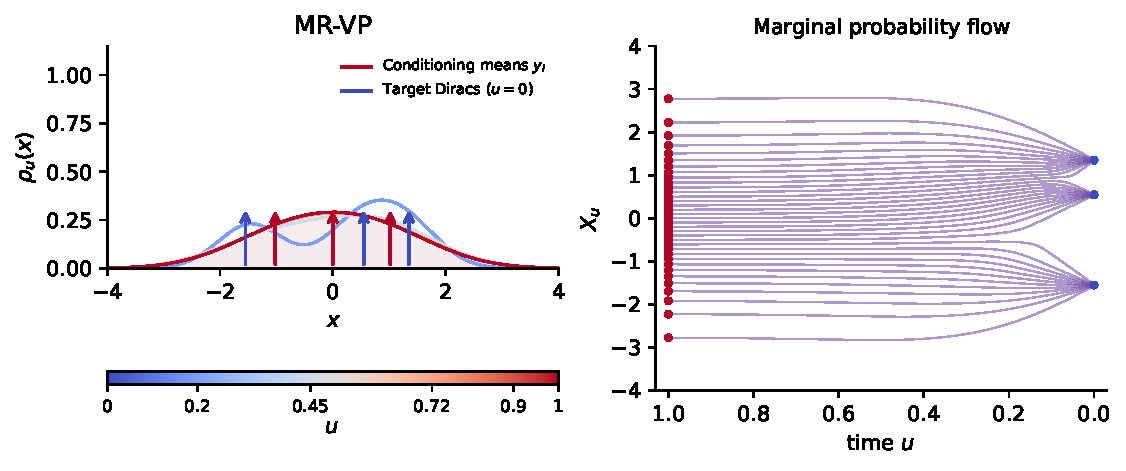
\includegraphics[width=0.95\linewidth]{plots/simulation_free/bridge_1d_mr_vp.pdf}\label{fig:mrvp-mixture}}
\caption{One-dimensional \acs{MR-VP} paths for the same three target Diracs. Left: forward densities; right: marginal probability-flow trajectories towards the data at $u=0$. In (a), $Y=0$ for every data point and the source approaches $\gN(0,1)$. In (b), each target point $x_i$ is paired with a fixed conditioning point $y_i$, with conditional law $Y\mid X=x_i\sim\delta_{y_i}$. The source approaches $\frac{1}{3}\sum_i\gN(y_i,1)$. The conditioning Diracs specify the reversion means; the source itself is a Gaussian mixture. With the finite noise schedule shown, these source distributions are approximate.}
\label{fig:mean_reverting_sde}
\end{figure}

Often, the properties of the source distribution must be designed for a given task. This means specifying how the path evolves through $u$ is important, as the terminal boundary of the path is the source distribution of the generative model. A key characteristic of a Gaussian is the mean and variance. The path described in this section uses mean-reversion to control the terminal mean, and variance preservation to influence a source with unit variance. In other words, a time-inhomogeneous Ornstein-Uhlenbeck process.

First, define a function of $u$, known as a  $\beta$-schedule
\[
\beta(u)\coloneqq\beta_{\min}+\bigl(\beta_{\max}-\beta_{\min}\bigr)u.
\]
This schedule is used to construct a variance preserving \acs{SDE}
\[
\dd \rmX \coloneqq \frac{1}{2}(\mY - \rmX_u)\beta(u) \dd u + \sqrt{\beta(u)} \dd\rmW_u.
\]
A consequence of the $\beta$-schedule is that the strength of the mean-reversion towards $\mY$ increases linearly with $u$. Secondly, the rate at which diffusion contributes variance increases linearly with $u$. Together, the drift and diffusion terms are balanced by the coefficients $\frac{1}{2}\beta(u)$ and $\sqrt{\beta(u)}$, resulting in a terminal distribution $p_1$ with approximately unit covariance given $\mY$.


Substituting drift and diffusion into \eqref{eq:sderev}, the reverse \acs{SDE} is
\[
\dd \rmX = \left(\frac{1}{2}(\mY - \rmX_u) - \nabla\log p_u(\rmX_u)\right)\beta(u) \dd u + \sqrt{\beta(u)} \dd\bar\rmW_u.
\]
A useful property of this \acs{SDE} is that its closed-form solution is known for an initial $\rmX_0$:
\[
p_u(\rmX_u|\rmX_0) = \mathcal N(\rmX_u;\rmM(\rmX_0,u,\mY),\mathsf\Sigma(u)),
\]
\[
\rmM(\rmX_0,u,\mY) = \left(1-e^{-\frac{1}{2}\int_0^u\beta(s)\dd s}\right)\mY +e^{-\frac{1}{2}\int_0^u\beta(s)\dd s}\rmX_0,
\]
\[
\mathsf\Sigma(u) = \left(1-e^{-\int_0^u\beta(s)\dd s}\right)\tI,
\]
\[
\int_0^u\beta(s)\dd s = \beta_{\min}u + \frac{1}{2}(\beta_{\max}-\beta_{\min})u^2.
\]
This allows sampling from $p_u$ instead of solving \eqref{eq:sdesolv}, resulting in \textit{simulation-free} training.

An important simplification here is the use of an isotropic covariance matrix. There are situations where the data might be better learned with non-isotropic Gaussians \citep{dhariwalDiffusionModelsBeat2021}, or non-diagonal \citep{xia2026improved,voleti2022scorebaseddenoisingdiffusionnonisotropic}. Such extra generalisations are beyond the topic of this thesis, but remain important to acknowledge.


The diffusion construction above uses a Gaussian terminal distribution centred at $\mY$ for all $\rmX_0$. This choice can be restrictive for tasks whose source distribution is itself a data distribution. There are many tasks that are better described as finding a coupling between two data distributions. Some examples include image super resolution, speech noise suppression, and \acf{TTS}.

In these cases, the mixture path follows a coupled law $\pi(\rmX,\rmY)$, the boundaries become mixtures of Gaussians on both sides, and a path becomes conditional on $\rmY$. Examples of paths between paired endpoints are shown in \figref{fig:path-overview}. The language around ``conditional paths'' now becomes tricky. This thesis uses ``conditional'' to refer to ``conditional to $\rmX_0$''.

There are other methods that directly answer such coupled problems. These methods are motivated by optimal transport theory. Specifically they are concerned with dynamic \acs{OT}, which aims to find the minimum energy vector field that describes a transport between two distributions. \Secref{sec:schr} and \secref{sec:icfm} cover \acs{SB} and \acs{FM}, respectively.

\subsection{Schr\"odinger bridges}
\label{sec:schr}


The original \acs{SB} problem describes paths between two observations at $u=0$ and $u=1$. The paths are required to have specified endpoint marginals and are compared with a reference path law $P_\mathrm{ref}$. The Schr\"odinger bridge minimises path-space Kullback--Leibler divergence subject to those marginal constraints:
\[
\min _{P\in\mathcal{P}_{\left[0,1\right]}(p_0,p_1)} D_{\text{KL}}(P\Vert P_\mathrm{ref}).
\]
Under standard regularity conditions, the solution can be represented using positive Schr\"odinger potentials $\Psi_u$ and $\hat\Psi_u$ in the forward and reverse \acsp{SDE}
\[
\dd\rmX \coloneqq \left[\rmF(\rmX,u) + g^2(u)\nabla\log\mPsi_u\right]\dd u + g(u)\dd \rmW_u,
\]
\[
\dd\rmX \coloneqq \left[\rmF(\rmX,u) - g^2(u)\nabla\log\hat\mPsi_u\right]\dd u + g(u)\dd \hat\rmW_u.
\]
The time-$u$ marginal density is proportional to the product $\hat\Psi_u\Psi_u$; the proportionality constant is fixed by normalisation.
Assume linear drift $\rmF(\rmX)=f(u)\rmX$ and Gaussian boundaries
\[
p_0=\gN(\rmX,\epsilon_0^2\tI) \quad p_1=\gN(\rmY,\epsilon_1^2\tI),
\]
where $\epsilon_1=e^{\int_0^1f(u)\dd u}\epsilon_0$. As $\epsilon_0\rightarrow 0$, the closed-form solution \citep{bunne2023schrodinger} is expressed as
\[
\hat\mPsi_u=\gN\left(e^{\int_0^uf(s)\dd s}\rmX,e^{2\int_0^uf(s)\dd s}\int_0^u\frac{g^2(s)}{e^{2\int_0^sf(v)\dd v}}\dd s\tI\right),
\]
\[
\mPsi_u=\gN\left(\frac{e^{\int_0^uf(s)\dd s}}{e^{\int_0^1f(s)\dd s}}\rmY,e^{2\int_0^uf(s)\dd s}\left[\int_0^1\frac{g^2(s)}{e^{2\int_0^sf(v)\dd v}}\dd s - \int_0^u\frac{g^2(s)}{e^{2\int_0^sf(v)\dd v}}\dd s\right]\tI\right).
\]
Given that the forward $\mPsi$ is guaranteed to have mean $\rmY$ at $u=1$, and the reverse is guaranteed to have mean $\rmX$ at $u=0$, the solution can be simplified by considering reference paths with zero drift $f(u)=0$, leading to
\[
\hat\mPsi_u=\gN\left(\rmX,\int_0^ug^2(s)\dd s\tI\right),
\]
\[
\mPsi_u=\gN\left(\rmY,\int_0^1g^2(s)\dd s - \int_0^ug^2(s)\dd s\tI\right);
\]
the mean and covariance of the solution $p$ are
\[
\label{eq:bridge-mean}
\rmM(\rmX,\rmY,u)=\left(1-\frac{\int_0^ug^2(s)\dd s}{\int_0^1g^2(s)\dd s}\right)\rmX + \left(\frac{\int_0^ug^2(s)\dd s}{\int_0^1g^2(s)\dd s}\right)\rmY,
\]
\[
\label{eq:bridge-covariance}
\tSigma = \int_0^ug^2(s)\dd s\left(1-\frac{\int_0^ug^2(s)\dd s}{\int_0^1g^2(s)\dd s}\right)\tI.
\]
This solution is related to the diffusion framework described in \secref{sec:diffusion-paths}. Bridge paths can connect prescribed endpoint distributions, and this Gaussian example has zero conditional variance at its boundaries. This property alone does not establish lower prediction error or better generalisation than a mean-reverting \acs{SDE}.

An important distinction with supervised learning is that samples from the boundaries are paired
\[
(\rmX^{(i)},\rmY^{(i)})\sim\pi(\rmX,\rmY).
\]


\subsection{Variance-exploding bridge}
Above has discussed that an \acs{SB} has two important features: boundary constraints and a reference path. Here an example reference path will be given. The path in question is \textit{variance-exploding}, motivated by results in speech enhancement \citep{jukic2024schr,gonzalez2023investigating}. This path continuously increases variance with $u$, an interesting property since the \acs{SB} solution must have zero variance at $u=1$. This conflict allows a path with high variance while ensuring the source distribution is exact, although the benefits of high variance are largely unknown but likely regularise neural network optimisation.

 A purely variance-exploding reference process has zero drift
\[
\dd \rmX \coloneqq \bm 0 \dd u + \sqrt{ck^{2u}}\dd\rmW_u.
\]
For clarity, define accumulated variance of the reference process
\[
\sigma_u^2 \coloneqq \int_0^ug^2(s)\dd s = \frac{c(k^{2u}-1)}{2 \log k}.
\]
Substituting this accumulated variance into \eqref{eq:bridge-mean} and \eqref{eq:bridge-covariance} yields a conditional probability path
\[
  \label{eq:sb_mean_variance}
  \rmM_u(\rmX_0, \rmY) = \left(1 - \frac{\sigma_u^2}{\sigma_1^2}\right) \rmX_0 + \frac{\sigma_u^2}{\sigma_1^2} \rmY,
\]
\[
\tSigma(u) = \sigma_u^2 \left(1 - \frac{\sigma_u^2}{\sigma_1^2}\right)\tI.
\]



\begin{figure}[tb]
\centering
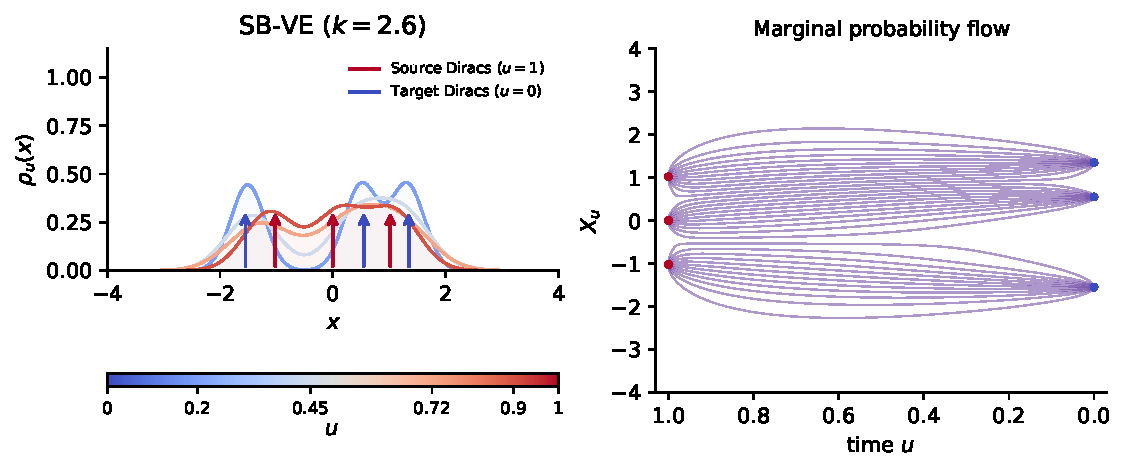
\includegraphics[width=\linewidth]{plots/simulation_free/bridge_1d_sb_ve_k2.6.pdf}
\caption{Variance-exploding bridge with $k=2.6$. The conditional variance vanishes at both endpoints.}\label{fig:schrodinger_bridge}
\end{figure}

\Figref{fig:schrodinger_bridge} shows a one-dimensional example. Reading from $u=0 \rightarrow 1$, the path is a mixture of Gaussians with increasing variance to a point, and then returning to zero around the data points to satisfy the endpoint constraints. This evolution of variance between exact endpoints is characteristic of \acs{SB}, diffusion evolves variance without reverting to zero, and flow matching keeps variance constant for every $u$.

\begin{figure}[tb]
\centering
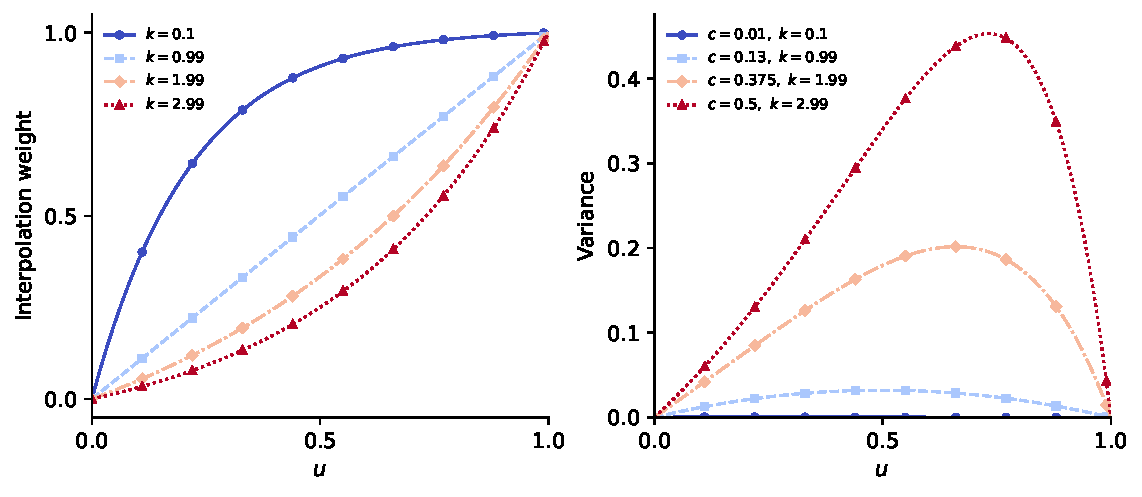
\includegraphics[width=\linewidth]{plots/simulation_free/k_c_plot.pdf}
\caption{\acs{SB-VE} interpolation weight and conditional variance as functions of depth $u$. Left: varying $k$ with $c=0.4$; the normalised weight is independent of $c$ and approaches linear interpolation as $k\rightarrow1$. Right: the displayed pairs of $c$ and $k$ vary together. Variance vanishes at both endpoints; at fixed $k$, it scales linearly with $c$.}
\label{fig:sb_kc}
\end{figure}

As illustrated in \figref{fig:sb_kc}, the speed of interpolation for the variance-exploding bridge the mean $\rmM$ tends to linear interpolation as $k\rightarrow1$, and is inhomogeneous otherwise. The variance $\tSigma$ is $0$ at the boundaries and increases towards the centre. This dynamic movement can make deep learning more difficult. Given that this variance is artificial, it is important to determine the benefits of this noise. Next, this thesis uses flow matching as an example of a path with less ``artificial noise''.



\subsection{Path variance and flow matching}
\label{sec:icfm}
\label{sec:sbsv}
Related simulation-free approaches emerged in 2022--2023. Liu, Gong, and Liu introduced rectified flow, using regression on straight interpolations and repeated rectification to straighten learned trajectories (preprint September 2022; \citealp{liuFlowStraightFast2022a}). Albergo and Vanden-Eijnden developed stochastic interpolants with a quadratic velocity objective (preprint September 2022; \citealp{albergoBuildingNormalizingFlows2023}). Lipman, Chen, and colleagues introduced flow matching through conditional probability paths (preprint October 2022; \citealp{lipman2023flow}). Tong and colleagues subsequently generalised conditional flow matching to arbitrary source distributions and endpoint couplings, including minibatch optimal-transport couplings (preprint February 2023; \citealp{tongImprovingGeneralizingFlowbased2024}).
\begin{figure}[tb]
\centering
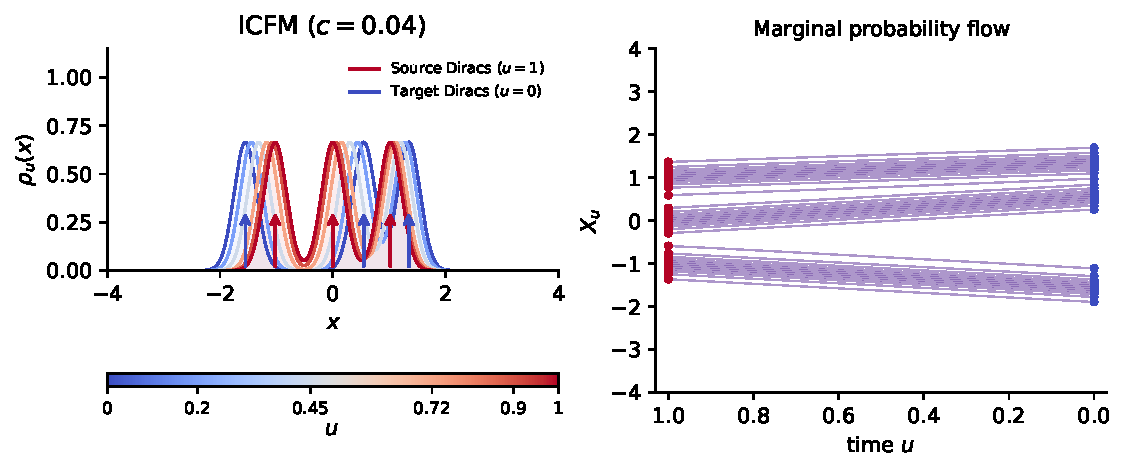
\includegraphics[width=\linewidth]{plots/simulation_free/bridge_1d_icfm_c0.04.pdf}
\caption{Conditional path for flow matching: linear interpolation with constant covariance $0.04\tI$, including at the endpoints.}\label{fig:conditional_flow_matching}
\end{figure}


For conditional flow matching, the path considered here uses a linearly interpolating mean and constant covariance. The motivation is that linear interpolation has constant velocity, which is optimal from a kinetic energy point of view \citep{mccannConvexityPrincipleInteracting1997}, and reduces input variance to the neural network during optimisation.

\[
\frac{\dd}{\dd u}\rmM_u=\rmY-\rmX_0.
\]
The conditional mean follows a straight path, with $\frac{\dd}{\dd u}\rmM_u=\mY-\rmX_0$. The target $\rmX_0-\mY$ below is therefore the velocity in the reverse depth direction (from $u=1$ towards $u=0$). This is McCann's displacement interpolation only in the zero-noise limit and when the endpoint coupling is optimal for the transport cost. The conditional path is described as
\[
\rmM(\rmX_0,\rmY,u) = u\rmY + (1-u)\rmX_0 \quad \tSigma(u)= c\tI.
\label{eq:icfm_mean_variance}
\]

The constant covariance used here is a choice of probability path, rather than a requirement of flow matching. Other constructions use depth-dependent conditional covariance.

For $c>0$, the conditional endpoints retain covariance $c\tI$ rather than being exact point masses. The purpose of this covariance is to satisfy Gaussian assumptions and perhaps act as regularisation as well.

For the sake of ablation, this thesis proposes \acs{SB-SV}. This path shares \acs{SB} interpolation with \acs{FM} variance. The goal here is to observe the practical implications of interpolation and variance design. \acs{SB-SV} subsumes \acs{FM} because it is possible to construct an \acs{SB-SV} path with almost linear interpolation (recall \figref{fig:sb_kc}).

\begin{table}
    \centering
    \begin{tabular}{cccc}
    \toprule
          &\acs{MR-VP}&  \acs{SB-VE}& \acs{ICFM}\\
         \midrule
         Exact interpolation &n&  y& n\\
         Static variance &n&  n& y\\
         Static gradient &n&  n& y\\
         \bottomrule
    \end{tabular}
    \caption{Comparison of the \acs{SB-VE} and \acs{ICFM} conditional paths. Exact interpolation refers to unsmoothed endpoints; static gradient refers to the conditional mean velocity.}
    \label{tab:sb-icfm-path-properties}
\end{table}

\subsection{Optimal transport}
\note{Review the transport claims below, including the relation between flow matching, fixed endpoint couplings, and minimum kinetic energy, and complete the unfinished equations.}
\ainote{The minimum-energy claim needs qualification. Straight, constant-speed paths minimise the action for each fixed endpoint pair, but a prescribed data coupling need not minimise transport cost over all couplings. Moreover, the marginal velocity learned by flow matching averages conditional velocities at each intermediate state, so its trajectories need not preserve the original pairing or remain straight. General flow matching therefore does not automatically solve dynamic optimal transport; the optimal-coupling and vanishing-smoothing assumptions matter \citep{tongImprovingGeneralizingFlowbased2024}. Describe the Schr\"odinger bridge as minimising relative entropy to a specified reference path law, with the connection to quadratic transport made under the corresponding Brownian-reference and small-noise assumptions. The two unfinished expressions below concern conditional marginalisation rather than transport optimality. If this is the intended model factorisation, a complete identity is
\[
p_0(\rmX_0\mid\rmY)
=\int p_{0\mid1,Y}(\rmX_0\mid\mX_1,\rmY)
\,p_{1\mid Y}(\mX_1\mid\rmY)\dd\mX_1.
\]
State the source law separately. Conditioning the first factor only on the source sample would require an additional conditional-independence assumption. No integration over the joint data law is needed in this identity.}
From an \acf{OT} perspective, \acf{FM} can be seen as a solution to the dynamic \acs{OT} problem, and \acs{SB} is an entropic regularisation of this. When dealing with paired endpoints, the coupling is already resolved. With this, only the minimum kinetic energy component of the dynamic \acs{OT} problem is optimisable, of which \acs{FM} fully addresses but diffusion models and \acs{SB} address with added noise. The benefit of added noise is an open topic.
\[
p_0(\rmX_0|\rmY)=\iint p_0(\rmX_0|\rmX_1)\gN(\dd\rmX_1|\rmY,\tSigma_1)\dd \pdata(\rmX_0,\rmY).
\]
\[
p(x0|x1)p(x1|y)
\]
% SVM integrals,
% p(x0|y)p(y)dx0dy
%loss = log p d data
% int int p(x0|)p(x1)p(z)dxdz dl? inverse wishart is distribution given length

\section{Simulation-free learning objectives}
\label{sec:learning-objectives}

This work now turns to how the parameters of these generative models are optimised. So far only the (conditional) target paths have been explained. The technique for training from a target path involves training a neural \acs{ODE} to predict the vector-field that describes the target path without reliance on endpoint conditioning. The objective functions for the neural networks are score-matching, data prediction and flow-matching for diffusion, \acs{SB} and \acs{FM} models respectively. It is possible to rewrite score-matching and flow-matching as a data prediction objective.

Simulation-free training is analogous to teacher-forcing. An instantaneous point from a reference path is sampled, and input to the estimator. A sufficiently trained model will align with the reference path, much like a sequence model aligning to likely sequences.

\subsection{Score and clean-data prediction}


The marginal score is typically intractable, but for a Gaussian transition the conditional score $\nabla\log p_{u|0}(\rmX_u|\rmX_0)$ is available in closed form. Although this target depends on $\rmX_0$, a network that receives only $(\rmX_u,u)$ can learn the marginal score by conditional score matching. With an unrestricted function class and samples from the stated training distribution, the population regression optimum is the marginal score \citep{song2021sde}. The objective is
\[
\label{eq:score-objective}
\vtheta^\ast\in\underset{\vtheta}{\arg\min}\;\E_{\ru,\rmX_0,\rmX_\ru}\left\lVert\rmS_\vtheta(\rmX_\ru,\ru)-\nabla_{\rmX_\ru}\log p_{\ru|0}(\rmX_\ru|\rmX_0)\right\rVert_2^2.
\]
Here $\ru\sim\gU(0,1)$ is the random depth, $\rmX_0$ is sampled from the empirical data distribution $\ptrain(\rmX_0)$, and $\rmX_\ru$ is sampled from its conditional transition law $p_{\ru|0}(\rmX_u|\rmX_0)$.
By sampling $\rmX_1\sim p_1$ and integrating the probability-flow \acs{ODE} backwards with the estimated marginal score, data samples can be generated (see \secref{sec:probability-flow}). Note how depth is optimised at the ``infinite layer limit'', and a random ``layer'' is optimised per sample per optimisation step.


In the case where the \acs{SDE} has a closed-form Gaussian solution, the conditional score becomes easy to compute. Assume that the conditional probability path is Gaussian:
\[
p_{u|0}(\rmX_u|\rmX_0) = \gN(\rmX_u;\rmM(\rmX_0,u),\mathsf\Sigma(u)),
\]
where $\rmM$ is the mean and $\tSigma$ is the covariance. Write
$\rmX_u=\rmM(\rmX_0,u)+\tSigma(u)^{1/2}\rmZ$, where $\rmZ\sim\gN(\bm0,\tI)$. The conditional score is then
\[
\nabla_{\rmX_u}\log p_{u|0}(\rmX_u|\rmX_0) = -\tSigma(u)^{-\frac{1}{2}}\rmZ.
\]
This form gives a simple training target for the score estimator.

An alternative to predicting the score is to predict the target data given the noisy sample:
\[
\vtheta^\ast\in\underset{\vtheta}{\arg\min}\;\E_{\ru,\,\rmX_0,\,\rmX_\ru}\left\lVert\rmD_\vtheta(\rmX_\ru,\ru)-\rmX_0\right\rVert_2^2,
\]
where $\ru,\rmX_0$ and $\rmX_u$ are sampled from the same laws as in \eqref{eq:score-objective}.
For the special case $\rmX_u=\rmX_0+u\rmZ$, with $\rmZ\sim\gN(\bm0,\tI)$, the optimal denoiser satisfies
\[
\nabla_{\rmX_u}\log p_u(\rmX_u)=\frac{\rmD^*_\vtheta(\rmX_u,u)-\rmX_u}{u^2}.
\]
For the general affine Gaussian transition $\rmX_u=a_u\rmX_0+b_u+\tSigma(u)^{1/2}\rmZ$ \note{(do we need $\rmY$ here?)}, the corresponding identity is
\[
\nabla_{\rmX_u}\log p_u(\rmX_u)=\tSigma(u)^{-1}\left(a_u\rmD^*_\vtheta(\rmX_u,u)+b_u-\rmX_u\right).
\]
These identities apply to the population-optimal denoiser; a trained network only approximates that optimum. The denoiser objective predicts the clean target at every noise level \citep{karras2022elucidating}.
\ainote{Reply to the question about $\rmY$ above: it is unnecessary when $b_u$ is deterministic and common to all samples. For a paired or encoder-conditioned path, write $b_u(\rmY)$ and condition both the score and denoiser on $\rmY$:
\[
\nabla_{\rmX_u}\log p_u(\rmX_u\mid\rmY)
=\tSigma(u)^{-1}\bigl(a_u\rmD^*_\vtheta(\rmX_u,u,\rmY)
+b_u(\rmY)-\rmX_u\bigr).
\]
Here the optimal denoiser is the conditional mean of $\rmX_0$ given $(\rmX_u,u,\rmY)$, and the covariance must be invertible. If $\rmY$ is random and unobserved, its offset must also be averaged conditionally on $\rmX_u$; inserting a particular $\rmY$ into a marginal-score identity is not valid.}




\subsection{Bridge data prediction}
For \acs{SB} case, a data-prediction objective regresses the clean endpoint from a path sample:
\[
\vtheta^\ast\in\underset{\vtheta}{\arg\min}\;\mathbb E_{(\rmX_0,\rmY),\ru,\rmX_\ru}\left[\left\|\rmD_\vtheta(\rmX_\ru\mid\rmY,\ru)-\rmX_0\right\|^2\right].
\]
In this expectation, paired endpoint data is sampled from a data law $(\rmX_0,\rmY)\sim\pi$, draw an independent time $\ru\sim U(0,1)$, and then sample the intermediate state $\rmX_\ru\sim p_{\ru\mid 0,Y}(\cdot\mid\rmX_0,\rmY)$ from the bridge/forward transition conditional on $(\rmX_0,\rmY)$.


\subsection{Flow matching by velocity prediction}
\label{sec:flow-matching-objective}
For the linear interpolation path in \secref{sec:icfm}, conditional flow matching regresses the reverse-depth velocity:
\[
\label{eq:flow-matching-objective}
\vtheta^\ast =\arg\min_\vtheta\mathbb E_{(\rmX_0,\rmY),\ru,\rmX_\ru}\left[\left\|\rmF_\vtheta(\rmX_\ru\mid\rmY,\ru)-(\rmX_0 -\rmY)\right\|^2\right].
\]
Similar to the \acs{SB} objective, sample paired endpoint data $(\rmX_0,\rmY)\sim\pi$, draw an independent time $\ru\sim U(0,1)$, and then obtain $\rmX_\ru$. \Eqref{eq:flow-matching-objective} assumes a linear interpolating path $\nabla_u \rmX=\rmX_0-\rmY$, although the design space supports many conditional vector fields and manifolds e.g. Riemannian flow matching.


\begin{table}[tb]
\centering\small
\begin{tabular}{lll}
\toprule
Path & Prediction target & Inference \\
\midrule
Diffusion & Score or clean data & Probability-flow \acs{ODE} \\
Variance-exploding bridge & Clean endpoint & Bridge sampler or direct prediction \\
Flow matching (linear path) & Reverse velocity & \acs{ODE} or direct prediction \\
\bottomrule
\end{tabular}
\caption{Path, prediction, and inference choices considered in this chapter.}
\end{table}

\subsection{Architecture}
There are many ways to develop an architecture for the neural estimators $\rmS_\vtheta,\rmD,\rmF$. An identifying feature is that it depends on the depth variable $u$ in addition to the current sample $\rmX_u$. Two popular examples are NCSN++, an enhanced noise conditional score network, and the \acf{DiT}.

An NCSN++ \citep{song2021sde} is a modified U-Net \citep{ronneberger2015unet} with a learnt $u$-step embedding applied to each residual network block. The U-Net remains similar to the original implementation as a series of downsampling layers, a bottleneck, and then a series of upsampling layers. As with all convolutional neural networks, contextual dependence can only be modelled within the kernels receptive field.

A more modern approach is to use a \acs{DiT} \citep{peeblesScalableDiffusionModels2023}. A \acs{DiT} uses the transformer architecture with adaptive layer-norm to condition on the $u$-step. Since transformers are sequence models, modalities such as images require tokenisation. A strong method for this is to segment the image into patches and compute a patch embedding for each patch.

Both the NCSN++ and \acs{DiT} have a dimensionality-reduction step for features such as images and spectrograms. The NCSN++ uses down-sampling layers and \acs{DiT} uses patch embeddings. Such steps are interesting as the noise typically exists on the highest dimensional manifold whereas the data may lie on a much lower manifold e.g. an image of a blue sphere has much less variance than a standard normal sample. It might be the case that dimensionality reduction offers a denoising bias as it forces local correlation during the learned reverse process which is beneficial for a data-generating score network.

\section{Conditional generation}

An extension of the generative modelling task is conditional generation. This involves generating realistic data samples that are likely given a conditioning signal e.g. a text prompt. The notion of conditional distribution between two random variables becomes relevant here.
\[
p(\rmX|\vy)=?
\]
There are several ways to influence the generation process. One approach is to form a Bayesian score
\[
\nabla\log p_u(\rmX_u|\rvy)=\nabla\log p_u(\rmX_u) + \nabla\log p_u(\rvy|\rmX_u).
\]
$p_u(\rvy|\rmX_u)$ is known as the \textit{classifier}. Classifier-guided generation depends heavily on the quality of the classifier, which adds additional compute cost and often fails to generate high-quality samples. Two advanced techniques considered in this thesis are \acf{CFG} and mean-reverting \acsp{SDE}.
\subsection{Classifier-free guidance}
One option is to provide conditioning labels during training to optimise $\nabla\log p_u(\rmX_u|\rvy)$, e.g. the score network could use cross-attention to be informed by the conditioning signal. In doing so, the score estimator is at risk of overfitting to the labelled data and no longer providing a diverse density possible with the unconditional model.

\acs{CFG} overcomes this by training a conditional-unconditional mixture. The ``classifier'' can be written as
\[
\nabla_{\rmX_u}\log p_u(\rvy|\rmX_u) = \nabla_{\rmX_u}\log p_u(\rmX_u|\rvy) - \nabla_{\rmX_u}\log p_u(\rmX_u).
\]
Define $\omega$ to control the mixture of conditional and unconditional scores. The guided score is
\begin{align}
\nabla\log p_u(\rmX_u|\rvy,\omega)
&\coloneqq \nabla_{\rmX_u}\log p_u(\rmX_u) + \omega\bigl(\nabla_{\rmX_u}\log p_u(\rmX_u|\rvy) - \nabla_{\rmX_u}\log p_u(\rmX_u)\bigr) \\
&= \omega\nabla\log p_u(\rmX_u|\rvy) + (1-\omega)\nabla\log p_u(\rmX_u).
\end{align}
At $\omega=0$ this is the unconditional score; at $\omega=1$ it is the conditional score. Values $\omega>1$ extrapolate in the direction of the classifier gradient and give stronger guidance in the score field. This linear combination does not, by itself, establish the distribution produced by a particular sampler. The conditional and unconditional scores can be trained together by randomly replacing $\rvy$ with the null label $\oslash$ during training.

Figure~\ref{fig:cfg-comparison} illustrates the effect of $\omega$ using analytic conditional and unconditional scores.

\begin{figure}[htbp]
\centering
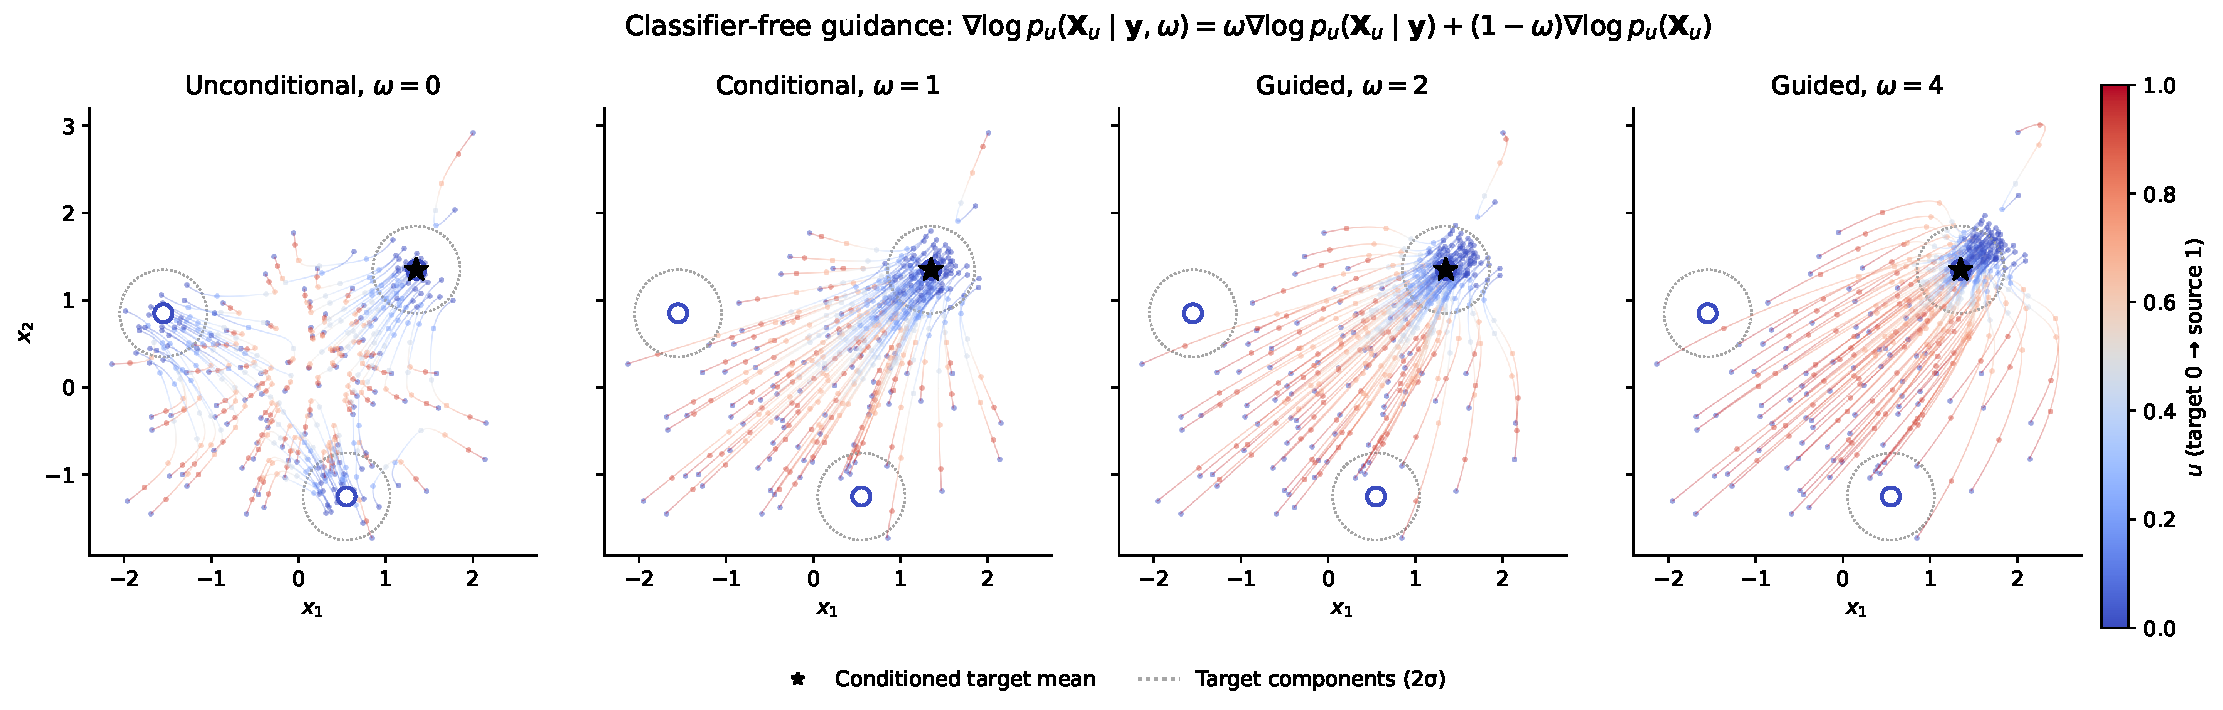
\includegraphics[width=\linewidth]{plots/simulation_free/cfg_comparison.pdf}
\caption{\acs{CFG} for a linear Gaussian interpolant, with guidance weights $\omega=0,1,2,4$. The unconditional target is an equal mixture of three Gaussian components; conditioning selects the upper-right component, marked by a star. All panels share 90 standard-normal source samples. Exact conditional and mixture scores define the guided velocity, integrated towards $u=0$ with 500 fourth-order Runge--Kutta steps. Colours indicate depth, and dotted circles show two standard deviations of the target components.}
\label{fig:cfg-comparison}
\end{figure}

\subsection{Mean reversion with conditional score}

In some cases, a coarse representation of the data is predictable, and diffusion is then used to refine the features. Here, the predicted coarse representation defines the mean of the terminal distribution
\[
\rmY\coloneqq \rmE_\vphi(\rvy),
\]
where $\rmE_\vphi$ is a deterministic encoder and $\rmY$ is the mean of $p_1$ conditional on $\rvy$.
Then for any \acs{SDE} with a mean reverting drift e.g. $\rmF(u)=\rmY-\rmX_u$ the score estimator is constrained to flows that revert to the mean $\rmY$.

This is a specific form of a two-sided \acs{SDE} where the encoder is incorporated into the paired data law $\pi$. The score estimator can then use the encoder output as a conditioning signal $\rmS_\vtheta(\rmX_u,u,\rmY)$. The use of an encoder-defined source mean is examined empirically in \chapref{ch:ll}.

Figure~\ref{fig:conditional-mrvp} illustrates this construction for three conditioning signals and their associated reversion means.

\begin{figure}[htbp]
\centering
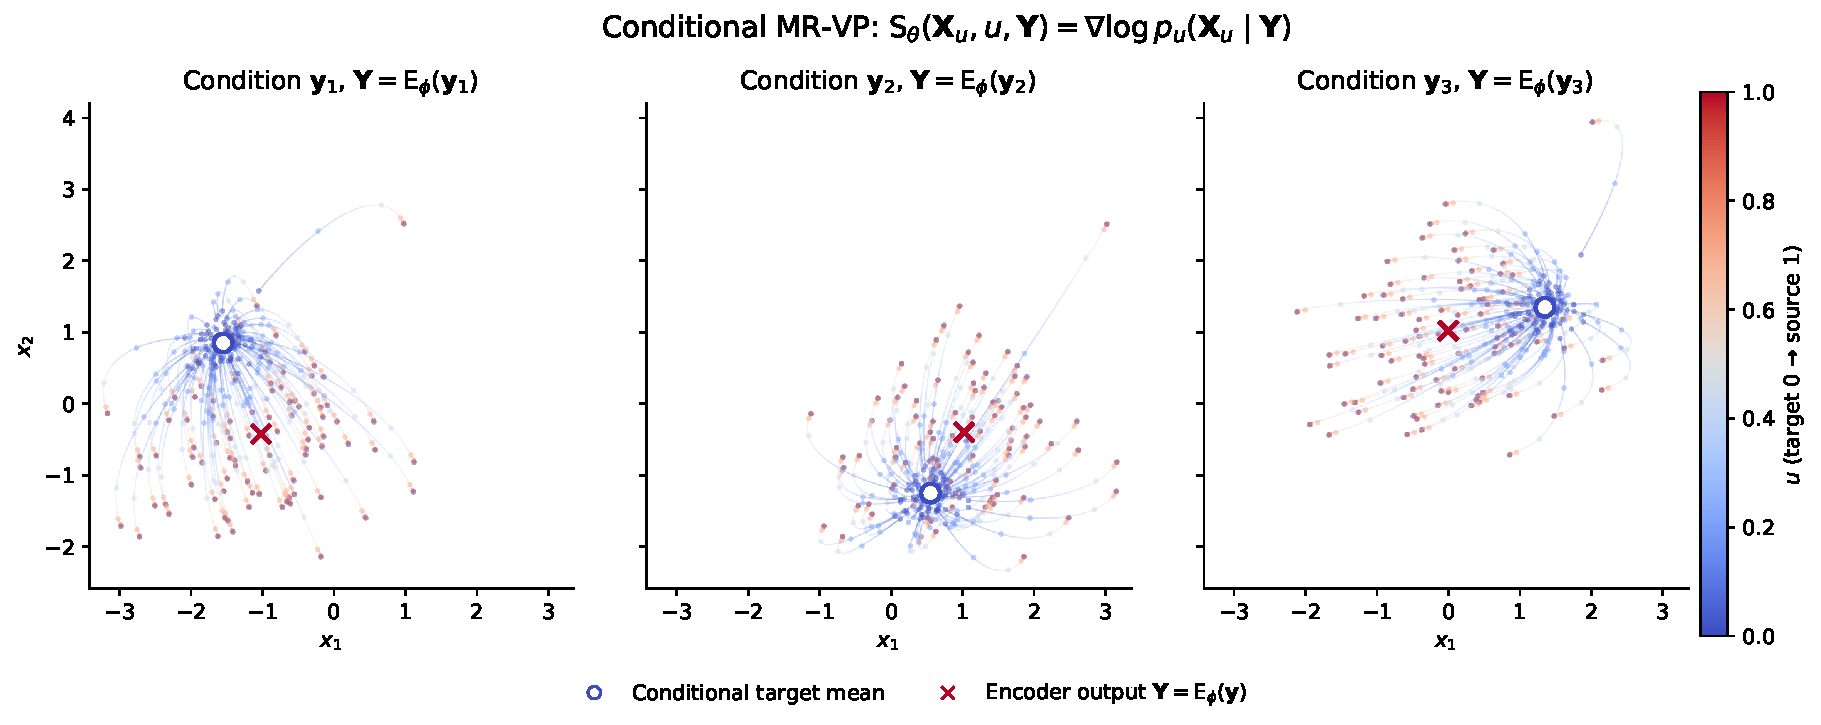
\includegraphics[width=\linewidth]{plots/simulation_free/conditional_mrvp.pdf}
\caption{Conditional \acs{MR-VP} probability-flow trajectories for three conditioning signals. Red crosses mark fixed illustrative encoder outputs $\rmY=\rmE_\vphi(\rvy)$, and blue circles mark the corresponding conditional target means. Each target is Gaussian with standard deviation $0.25$. All panels share 90 standardised noise draws and use analytic conditional scores with $\beta(u)=0.05+19.95u$, integrated towards $u=0$ with 1000 fourth-order Runge--Kutta steps. Initial samples follow the exact finite-depth marginal, approximately $\gN(\rmY,\tI)$. Colours indicate depth.}
\label{fig:conditional-mrvp}
\end{figure}




\section{Generation and likelihood evaluation}
\subsection{Probability-flow ODE}
\label{sec:probability-flow}

An attractive feature of \acsp{CNF} is that the change of variables formula becomes easier to compute. So far the reverse diffusion process has been presented in \acs{SDE} form, but for generation it is possible to use an equivalent deterministic \acs{ODE}
\[
\rmH_\vtheta(\rmX,u)\coloneqq \rmF(\rmX,u) - \frac{1}{2}g(u)^2\rmS_\vtheta(\rmX,u).
\]
This vector field defines the probability-flow \acs{ODE}.
For the variance preserving example, the probability-flow \acs{ODE} is
\[
\rmH_\vtheta(\rmX,u) \coloneqq \frac{1}{2}\left(\mY - \rmX-\rmS_\vtheta(\rmX,u)\right)\beta(u).
\]


For \acs{CFG}, apply the following probability flow \acs{ODE}
\[
\dd \rmX = \frac{1}{2}\left((\mY - \rmX_u) - \omega\mS_\theta(\rmX_u,u|\vy) + (\omega-1)\mS_\theta(\rmX_u,u|\oslash)\right)\beta(u)\dd u.
\label{eq:cfg}
\]
For mean reversion conditional on paired endpoints, $\rmY$ is a random variable linked to the opposite endpoint $\rmX_0$, unlike a global $\mY$ left as a design choice in \eqref{eq:cfg}. This represents a key difference between image and speech generative models examined in \chapref{ch:ll}.

The simplicity of flow-matching becomes clear when viewing its probability-flow \acs{ODE}
\[
\rmH_\vtheta(\rmX,u)\coloneqq\rmF_\vtheta(\rmX,u).
\]
As \acs{FM} optimises the least squares between the target path and parametric vector field, the flow estimator $\rmF_\vtheta$ is a drop-in probability flow \acs{ODE}. This is attractive as there is less separation between the training and generation process.




\subsection{Numerical sampling}

To retrieve data samples, the following reverse initial value problem must be solved with black-box \acs{ODE} solvers
\[
\rmX_0=\rmX_1 + \int_1^0\rmH_\vtheta(\rmX_u,u)\dd u.
\]
As stated earlier, this form of \acs{CNF} is a probability-flow \acs{ODE}. The lack of diffusion is useful as it constrains the input variance of the neural estimator $\rmS_\vtheta$.

A simple method is the Euler sampler
\[
\rmX_{u-h}=\rmX_u -\rmH_\vtheta(\rmX_u,u)h,
\]
where $h\leq 1$ is the step size. The number of steps required is $\frac{1}{h}$. This method has a fixed number of steps per solve. Typically, more steps improve accuracy, presenting a compute-accuracy trade-off.

There are many options for \acs{ODE} solvers. For example, the fourth-order Runge-Kutta method evaluates the vector-field four times per step \citep{Runge1895UeberDN,kutta1901beitrag}. Adaptive methods dynamically increase or decrease the step size under select criteria such as an error tolerance between fourth and fifth order evaluations \citep{dormandFamilyEmbeddedRungeKutta1980}. The development of diffusion models has lead to customised solvers for the generative task e.g. with special weighting schemes \citep{cheng2022dpmsolvr}.

A key area of research here is improving quality with less steps. Flow matching addresses this with straight paths, since less variation in the estimator target likely results in less variation in estimator error during sampling. Additionally, the speed of a path reduces variation, further removing potentially disruptive noise from the optimisation landscape. Rectified flows are one of the first to directly address this issue \citep{liuFlowStraightFast2022a}, and Peyre chapter XXX supports details for one-step generative models \citep{}.


\subsection{Bridge sampling}
The \acs{SB} problem requires a specific solver  derived from the \acs{SB} solution.
Recall the term in \acs{SB-VE}
\[
\sigma_u^2 \coloneqq \frac{c(k^{2u}-1)}{2 \log k}.
\]
The \acs{SB} path is then rewritten in terms of $\rmX_u$, $\rmX_0\coloneqq\rmD_\vtheta(\cdot)$, and $\rmX_1=\rmY$, which is a form of \acs{ODE} sampler
\[
\begin{aligned}
\mX_{u_{i-1}}
={}&
\frac{
    \sigma_{u_{i-1}}\sqrt{\sigma_1^2-\sigma_{u_{i-1}}^2}
}{
    \sigma_{u_i}\sqrt{\sigma_1^2-\sigma_{u_i}^2}
}
\mX_{u_i}
\\
&+
\frac{1}{\sigma_1^2}
\left(
    \sigma_1^2-\sigma_{u_{i-1}}^2
    -
    \frac{
        \sqrt{\sigma_1^2-\sigma_{u_i}^2}
        \sigma_{u_{i-1}}
        \sqrt{\sigma_1^2-\sigma_{u_{i-1}}^2}
    }{
        \sigma_{u_i}
    }
\right)
    \mD_\vtheta(\mX_{u_i},\rmY,u_i)
\\
&+
\frac{1}{\sigma_1^2}
\left(
    \sigma_{u_{i-1}}^2
    -
    \frac{
        \sigma_{u_i}\sigma_{u_{i-1}}
        \sqrt{\sigma_1^2-\sigma_{u_{i-1}}^2}
    }{
        \sqrt{\sigma_1^2-\sigma_{u_i}^2}
    }
\right)
\mY,
\end{aligned}
\]
for an increasing sequence of $u_i$. The denoiser is evaluated at the current state depth $u_i$. The formula is singular at the endpoint $u_i=1$, so an implementation needs an endpoint special case or a limiting update. Although there is nothing inherently wrong with a solver with complicated terms and coefficients, simplicity is desired when available, presented next.

\subsection{Direct data prediction}
An alternative to the \acs{SB}-\acs{ODE} proposed in this thesis is \acf{DDP}. In \secref{sec:learning-objectives} the data prediction objective is used to make the estimator well conditioned to clean data across all noise levels. An added benefit of the data prediction loss is that the estimator becomes a data predictor, and may be a sufficiently strong model without the need to solve an \acs{ODE}. Here the term ``direct data prediction'' is used to describe the use of a noise conditional model as a data predictor instead of an \acs{ODE}.

Direct data prediction with data prediction loss is
\[
\mX_0=\mD_\vtheta(\mY, \mY,1),
\]
and for flow-matching loss
\[
\mX_0=\mF_\vtheta(\mY, \mY,1) + \mY.
\]
Direct prediction evaluates the network once at the source depth. It does not integrate the intermediate path. For a path with nonzero endpoint variance, evaluation at the source mean should be distinguished from sampling the full source distribution.

There is an equivalence to a single Euler step of the \acs{SB}-\acs{ODE}, provided that the velocity at the source endpoint has the appropriate form. Integrating from $u=1$ to $u=0$ with a single Euler step gives
\[
{\rmX}_0=\rmY-\rmH_\vtheta(\rmY,\rmY,1).
\]
This coincides with direct data prediction when $\rmH_\vtheta(\rmY,\rmY,1)=\rmY-\rmD_\vtheta(\rmY,\rmY,1)$, or with the flow-matching expression above when $\vv_\vtheta(\mY,\mY,1)=-\mF_\vtheta(\mY,\mY,1)$. The equivalence therefore depends on the path parameterisation and the sign convention used for the predicted velocity; it does not hold automatically for every \acs{SB}-\acs{ODE}. Moreover, equivalence to a single Euler step does not imply equivalence to the fully integrated \acs{ODE}, which evaluates the evolving vector field along the intermediate path.




\subsection{Point-cloud illustrations of inference}
Figure~\ref{fig:inference-dirac-dirac} illustrates discrete inference trajectories for paired endpoints using \acs{MR-VP}, a Schr\"odinger bridge, and flow matching. These examples complement the opening probability-path overview by showing how the samplers move individual points. The stochastic source of \acs{MR-VP} becomes clear here, and the curves indicate wasted kinetic energy, which in turn requires the score estimator to support the dynamic movement.

During sampling, \acs{SB-VE} and \acs{FM} have equivalent linear trajectories, although their speeds differ. \acs{SB-VE} starts faster and slows as $u$ approaches $0$, \acs{FM} has constant speed. This observation shows that different training methods can result in similar paths during sampling. The \acs{SB} estimator must support evolving variance, which produce samples unlikely to be found during sampling. On the other hand, \acs{FM} provides a training path more similar to the sampling path, with equality as $c$ tends to $0$. It is possible to regain stochasticity in \acs{FM} by sampling from the Gaussian source rather than Dirac.

\begin{figure}[p]
\centering
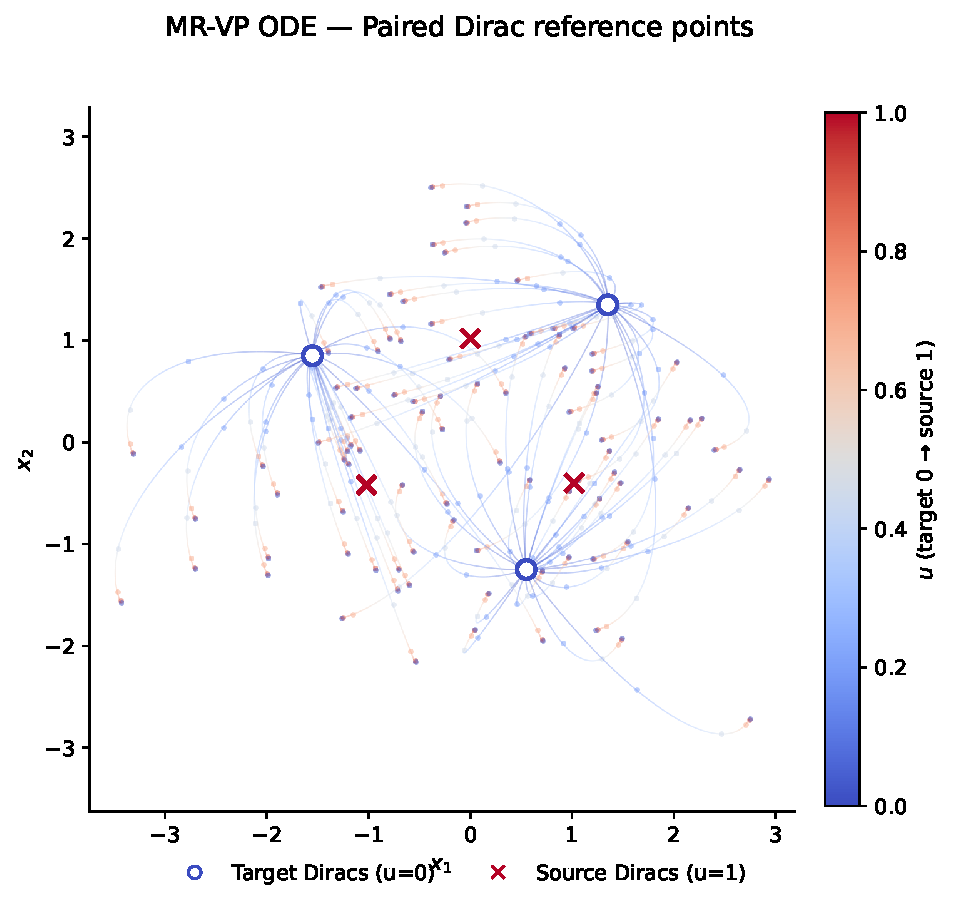
\includegraphics[width=0.48\linewidth]{plots/simulation_free/inference/dirac_dirac/mr_vp.pdf}\hfill
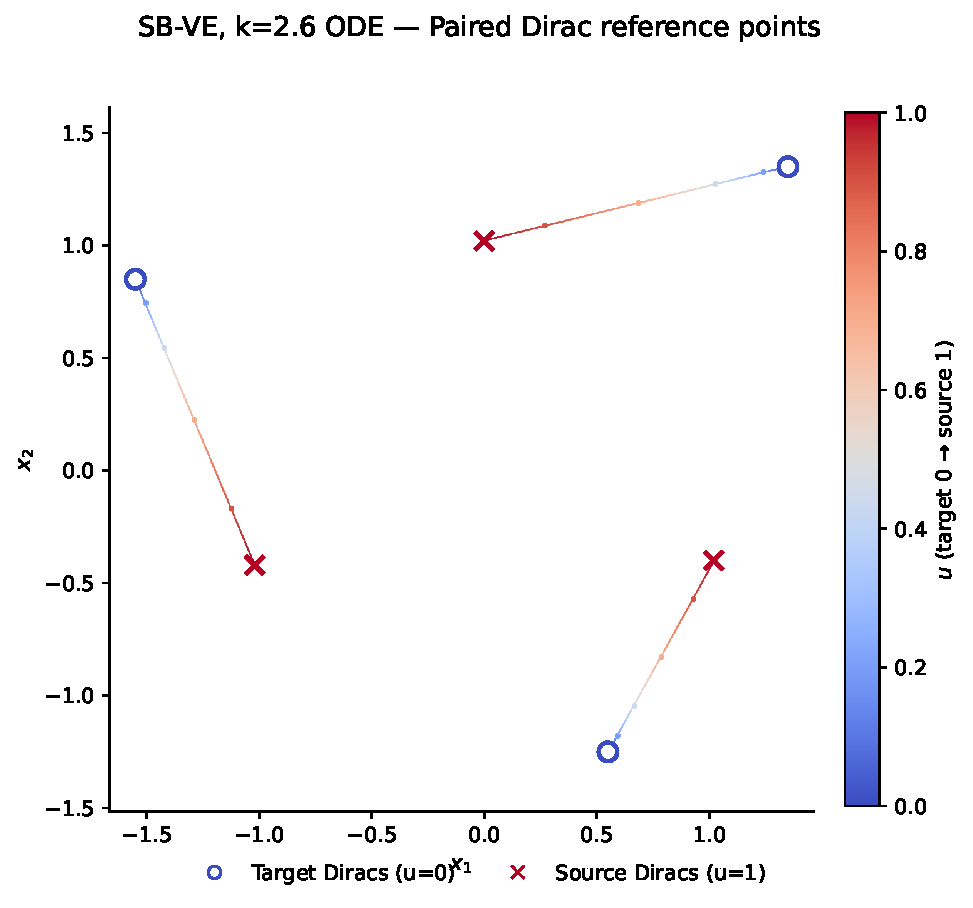
\includegraphics[width=0.48\linewidth]{plots/simulation_free/inference/dirac_dirac/sb_ve_k2.6.pdf}
\par\medskip
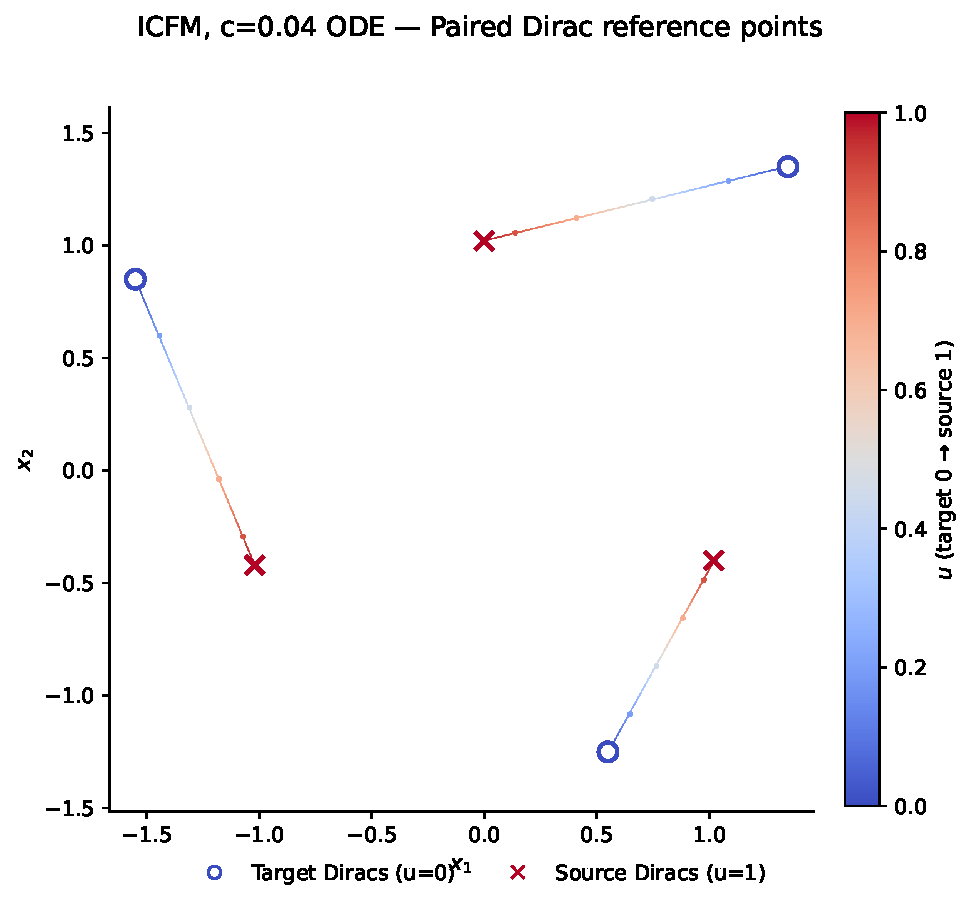
\includegraphics[width=0.48\linewidth]{plots/simulation_free/inference/dirac_dirac/icfm_c0.04.pdf}\hfill
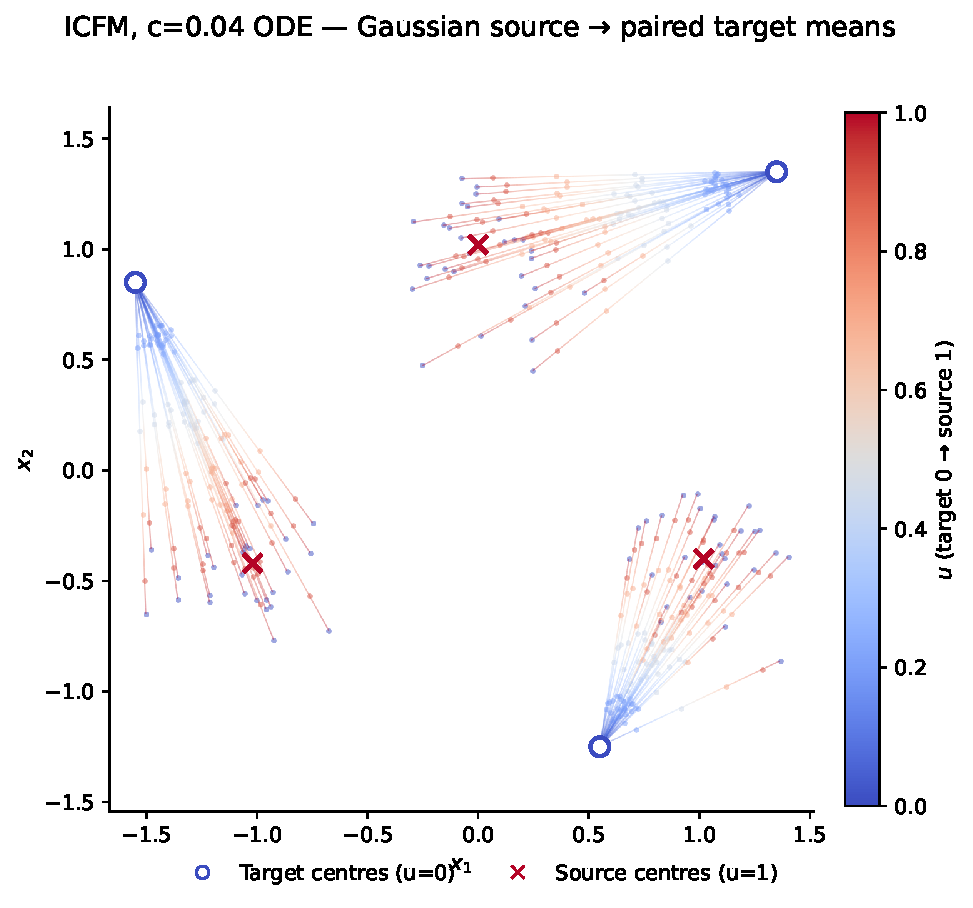
\includegraphics[width=0.48\linewidth]{plots/simulation_free/inference/paired_gaussians/icfm_c0.04.pdf}
\caption{Point-cloud inference for paired three-point distributions: \acs{MR-VP} (top left), \acs{SB-VE} with $k=2.6$ (top right), \acs{ICFM} with $c=0.04$ from observed source points (bottom left), and a Gaussian-source data-prediction illustration with $c=0.04$ (bottom right). Colours indicate depth, with generation proceeding towards $u=0$. Analytic conditional predictors and 100 discrete integration steps are used. Each source point uniquely identifies its target, so trajectories with identical starts coincide. \acs{MR-VP} starts from Gaussian noise about the conditioning mean; \acs{SB} and the bottom-left \acs{ICFM} example start at the observed source point. The bottom-right example starts from Gaussian noise with variance $c$ about each source point and follows straight lines to the paired target mean under the assumed data-prediction velocity. \acs{SB} integration begins at $u=1-10^{-4}$ to avoid singular endpoint coefficients.}
\label{fig:inference-dirac-dirac}
\end{figure}
\clearpage
\subsection{Likelihood evaluation}
\label{sec:likelihood-evaluation}
As discussed earlier, a property of normalising flows and \acsp{CNF} is likelihood of the density. In practice the log-likelihood is easier to compute. This function scores samples based on how likely they are to appear in the data distribution, a sample with higher log-likelihood implies the model assigns more probability to that sample. Computing likelihood of samples from the data $p_0(\rmX_0;\vtheta), \rmX_0\sim\pdata$ should be high, as we expect the model to correlate with the data distribution.

For a \acs{CNF}, the likelihood is
\[
\log p_0(\rmX_0;\vtheta)=\log p_1(\rmX_1) +\int_0^1\nabla_{\rmX_u}\cdot \rmH_\vtheta(\rmX_u,u)\dd u.
\]
The divergence can evaluated with a trace
estimator \citep{skillingEigenvaluesMegadimensionalMatrices1989,hutchinsonStochasticEstimatorTrace1989}
\[
\nabla_{\rmX}\cdot\rmH_\vtheta(\rmX,u)=\E_{\rmZ\sim\gN(\bm0,\tI)}\left[\rmZ^\top\nabla_{\rmX}\rmH_\vtheta(\rmX,u)\rmZ\right].
\]
Although score-based modelling is simulation-free, it removes the ability to maximise likelihood directly. Despite this, the learnt density outperforms non-continuous-depth alternatives \citep{song2021sde}. Interestingly, there are methods for maximum likelihood training \cite{songMaximumLikelihoodTraining2021}, yet these do not produce higher quality samples. Such research emphasises the fact that evaluating generative models is a non-trivial task.


A computable likelihood allows the model to be robustly evaluated. Despite this advantage, evaluating likelihood on practical tasks such as controllable image and speech generation is not commonplace. One reason for this is that it is common to report the average likelihood that the model assigns to samples from the data distribution. This is, of course, useful as it is expected that a model with higher likelihood better represents the data distribution, but viewing the average likelihood does not explain the calibration between the model and data e.g. are higher likelihood samples more likely according to the data. \Chapref{ch:ll} explores this gap.

\note{maybe mention theis et al here, maybe mention how we talk about log- and likelihood as the same}
\ainote{Yes: cite \citet{theisNoteEvaluationGenerative2016} to support distinguishing average held-out log-likelihood from perceptual sample quality and evaluating the intended application directly. That result does not itself establish the samplewise calibration property proposed here; define that property separately. State once that likelihood denotes the model density evaluated at an observation and that numerical results report its logarithm. The logarithm preserves individual density rankings, but averaging densities and averaging log-densities are different operations. For continuous observations, density is not point probability, so replace claims about the probability of an exact sample accordingly.}

\section{Task examples}
\note{This section needs a good look over.}
\ainote{The section needs three concrete additions: complete the empty text-to-image subsection with its conditioning signal and source law; distinguish discrete speech-length prediction from continuous generation at a fixed length; and specify a consistent observation model for noise suppression. For each example, identify the generated variable, conditioning variables, source distribution, and prediction target, then signpost the relevant experimental chapter. Present the Grad-TTS criticism as a hypothesis unless supported by a controlled comparison. The notes below address the length marginalisation and observation-model equations.}



\subsection{Text to image}

\subsection{Variable-length speech}
Some data types such as speech have an associated length $\rl$ with each sample $\rmX_0\in\R^{d\times\rl}$, where $d$ is the static dimension of the data e.g. number of Mel-spectrogram channels. This means the sampled terminal distribution $\hat p_1$ must also sample or predict a length to operate in. The length of a sample remains constantly for any $u$, though there exist methods such as jump diffusion that allow trans-dimensional $l$.

The statistical problem outlined in \acs{TTS} is to find the probability of an acoustic feature given a text

% working out bayes
\[
p(\rmX_0|\rvy)=\int_{\sZ_+} p(\rmX_0|\rvy,\rl)p(\rl|\rvy)\dd\rl.
\]
This density admits many $\rl$ since the same text since speaking rate adjusts the acoustic length. For a \acs{CNF}, boundaries of the same dimension must be defined

\[
p(\rmX_0|\rvy)=\int_{\sZ_+}\int_{\R^{d\times\rl}} p(\rmX_0|\rmX_1)p(\rmX_1|\rvy,\rl)p(\rl|\rvy)\dd\rmX_1\dd\rl.
\]

For an informed paired law, $\rmX_1$ can be marginalised by introducing an intermediate dimensionality expansion $\rmY$

\[
p(\rmX_0|\rvy)=\int_{\sZ_+}\iint_{\R^{d\times\rl}} p(\rmX_0|\rmX_1,\rmY)p(\rmX_1|\rmY)p(\rmY|\rvy,\rl)p(\rl|\rvy)\dd\rmX_1\dd\rmY\dd\rl.
\]

\note{Should $\int_{\sZ_+}$ be $\sum_{\sZ_+}$?}
\ainote{Yes, for a positive integer frame count use $\sum_{l=1}^{\infty}$ in all three expressions, and remove $\dd\rl$. Each summand is a density on its own space $\mathbb R^{d\times l}$, weighted by the length probability $p(l\mid\rvy)$; make the length component of the variable-length sample explicit. Retain $\rvy$ and $l$ in the decoder conditioning unless conditional independence has been justified. If the expanded encoder output is deterministic given text and length, $p(\rmY\mid\rvy,l)$ is a Dirac measure, so the integral over $\rmY$ reduces to evaluation at that output.}

Although Grad-TTS has shown success for diffusion, the framework is misaligned and becomes hard to work with. Grad-TTS simplifies the terminal distribution to a Gaussian with unit variance, which may be artificially increasing the difficulty of the problem. \note{Review the claim that unit source variance increases the difficulty of the problem.}
\ainote{This is a plausible experimental question, but unit covariance alone does not establish greater learning or sampling difficulty: its scale depends on feature normalisation, and performance also depends on the schedule, parameterisation, and solver. Grad-TTS derives a general diagonal terminal covariance, chooses the identity for simplicity, and also reports temperature-adjusted sampling \citep{popov21gradtts}, Section 3.1. Its source mean is already predicted from text. Qualify the criticism and test source variance while controlling the encoder, feature scale, architecture, training budget, and sampling budget. Distinguish changing the training path from changing only the inference temperature.}

% Author outline from gradtts.tex: Equations that describe speech enhancement.
\subsection{Paired endpoints for noise suppression}

Noisy speech is defined as a clean signal $\rmX$ convolved with a room impulse response $\mR$ and additive noise $\rmZ$
\[
\rmY \coloneqq \rmX\ast\mR + \rmZ.
\]
The goal of noise suppression is to retrieve $\rmX$ given $\rmY$.
\[
p(\rmX|\rmY)=\int p(\rmX|\rmY)p(\rmY|\rmX,\rmZ)\dd\rmZ.
\]
\note{Need to work on this.}
\ainote{The preceding integral is not a valid posterior factorisation: it repeats $p(\rmX\mid\rmY)$ on the right and supplies no noise prior. For a fixed known room response and additive noise independent of clean speech, define $p(\mY\mid\mX,\mR)=p_Z(\mY-\mX\ast\mR)$ and use Bayes' rule:
\[
p(\mX\mid\mY,\mR)
=\frac{p_Z(\mY-\mX\ast\mR)\,p_X(\mX)}
{\int p_Z(\mY-\mX'\ast\mR)\,p_X(\mX')\dd\mX'}.
\]
If the room response is unknown, marginalise it under a stated prior or joint model. The following formula for $q_1$ is a valid noisy marginal under the fixed-room and independence assumptions; define $q_0$, $q_1$, and $p_Z$ consistently. Finally, distinguish the observed noisy waveform from the artificial diffusion noise, and state whether the diffusion operates on waveforms or acoustic features.}

\[
q_1(\rmY)=\int p_z(\rmY - \rmX\ast\mR) q_0(\dd\rmX).
\]

The paired distributions motivate a conditional path.
Instead of a variance preserving \acs{SDE}, consider a variance exploding \acs{SDE}
\[
\dd\rmX\coloneqq\gamma(\rmY - \rmX_u)\dd u + \sqrt{ck^{2u}}\dd\rmW_u,
\]
\[
\rmM(\mY,\rmX,u;\gamma) = e^{-\gamma u}\rmX + (1- e^{-\gamma u})\mY \qquad \tSigma(u;\gamma,c,k) = \frac{c(k^{2u}-e^{-2\gamma u})}{2(\gamma + \log k)}\tI.
\]

When $\mR=I$, the flow-matching target also equals the additive-noise residual. With reverberation, this residual is $\rmY-\rmX=\rmX\ast\mR-\rmX+\rmZ$, so it is not the background noise alone:
\[
\rmY - \rmX = \rmX\ast\mR-\rmX+\rmZ.
\]


\section{Summary}
Simulation-free training combines a prescribed probability path with an accessible conditional regression target. Diffusion, bridge, and linear flow-matching path constructions provide different endpoint and variance choices. Score, clean-data, and velocity prediction connect these paths to inference procedures, while conditioning supports generation and paired transport.

Although the training objectives avoid numerical integration, likelihood evaluation generally requires integrating the learned dynamics and accumulating their divergence.

\Chapref{ch:ll} evaluates likelihood in practical diffusion models. \Chapref{ch:cfmse} examines paired paths, variance choices, and direct prediction for noise suppression.
